\documentclass[11pt,fleqn,a4paper]{book}

%%%%%%%%%%%%%%%%%%%%%%%%%%%%%%%%%%%%%%%%%
% The Legrand Orange Book
% Structural Definitions File
% Version 2.0 (9/2/15)
%
% Original author:
% Mathias Legrand (legrand.mathias@gmail.com) with modifications by:
% Vel (vel@latextemplates.com)
%
% This file has been downloaded from:
% http://www.LaTeXTemplates.com
%
% License:
% CC BY-NC-SA 3.0 (http://creativecommons.org/licenses/by-nc-sa/3.0/)
%
%%%%%%%%%%%%%%%%%%%%%%%%%%%%%%%%%%%%%%%%%

%----------------------------------------------------------------------------------------
%	VARIOUS REQUIRED PACKAGES AND CONFIGURATIONS
%----------------------------------------------------------------------------------------

\usepackage[top=3cm,bottom=3cm,left=3cm,right=3cm,headsep=10pt,a4paper]{geometry} % Page margins

\usepackage{graphicx} % Required for including pictures
\graphicspath{{img/}} % Specifies the directory where pictures are stored

\usepackage{titling} % Macros for title, author, etc
\usepackage{lipsum} % Inserts dummy text

\usepackage{tikz} % Required for drawing custom shapes

\usepackage[english,dutch]{babel} % English language/hyphenation
\usepackage{iflang}

\usepackage{enumitem} % Customize lists
\setlist{nolistsep} % Reduce spacing between bullet points and numbered lists

\usepackage{booktabs} % Required for nicer horizontal rules in tables

\usepackage{xcolor} % Required for specifying colors by name
\definecolor{maincolor}{RGB}{0,100,184} % Define the main color used for highlighting throughout the book

% Paragraph style: no indent, add space between paragraphs
\setlength{\parindent}{0em}
\setlength{\parskip}{1em}

%----------------------------------------------------------------------------------------
%	FONTS
%----------------------------------------------------------------------------------------

\usepackage{avant} % Use the Avantgarde font for headings
%\usepackage{times} % Use the Times font for headings
\usepackage{mathptmx} % Use the Adobe Times Roman as the default text font together with math symbols from the Sym­bol, Chancery and Com­puter Modern fonts
\usepackage{eurosym}

\usepackage{amsfonts}
\usepackage{amsmath}
\usepackage{amssymb}
\usepackage{textcomp}
\usepackage{wasysym}

\usepackage{microtype} % Slightly tweak font spacing for aesthetics
\usepackage[utf8]{inputenc} % Required for including letters with accents
\usepackage[T1]{fontenc} % Use 8-bit encoding that has 256 glyphs

%------------------------------------------------------------------------------
%	TITLE PAGE
%------------------------------------------------------------------------------

\newcommand{\thetitlepage}{%
\begingroup
\thispagestyle{empty}
\begin{tikzpicture}[remember picture,overlay]
\coordinate [below=12cm] (midpoint) at (current page.north);
\node at (current page.north west)
{\begin{tikzpicture}[remember picture,overlay]
\node[anchor=north west,inner sep=0pt] at (0,0) {
\includegraphics[width=\paperwidth]{background}}; % Background image
\draw[anchor=north] (midpoint) node [fill=maincolor,fill opacity=0,text=white,text opacity=1,inner sep=1cm]{\Huge\centering\bfseries\sffamily\parbox[c][][t]{\paperwidth}{\centering \thetitle\\[15pt] % Book title
{\Large \thedate}\\[20pt] % Subtitle
{\large \theauthor}}}; % Author name
\end{tikzpicture}};
\end{tikzpicture}
\vfill
\endgroup
}

%----------------------------------------------------------------------------------------
%	BIBLIOGRAPHY AND INDEX
%----------------------------------------------------------------------------------------

\usepackage[style=apa,backend=biber]{biblatex}
\usepackage{csquotes}
\DeclareLanguageMapping{dutch}{dutch-apa}
\addbibresource{bibliografie.bib} % BibTeX bibliography file
\addbibresource{voorbeelden.bib}
\defbibheading{bibempty}{}

\usepackage{calc} % For simpler calculation - used for spacing the index letter headings correctly
\usepackage{makeidx} % Required to make an index
\makeindex % Tells LaTeX to create the files required for indexing

%----------------------------------------------------------------------------------------
%	MAIN TABLE OF CONTENTS
%----------------------------------------------------------------------------------------

\usepackage{titletoc} % Required for manipulating the table of contents

\contentsmargin{0cm} % Removes the default margin

% Part text styling
\titlecontents{part}[0cm]
{\addvspace{20pt}\centering\large\bfseries}
{}
{}
{}

% Chapter text styling
\titlecontents{chapter}[1.25cm] % Indentation
{\addvspace{12pt}\large\sffamily\bfseries} % Spacing and font options for chapters
{\color{maincolor!60}\contentslabel[\Large\thecontentslabel]{1.25cm}\color{maincolor}} % Chapter number
{\color{maincolor}}
{\color{maincolor!60}\normalsize\;\titlerule*[.5pc]{.}\;\thecontentspage} % Page number

% Section text styling
\titlecontents{section}[1.25cm] % Indentation
{\addvspace{3pt}\sffamily\bfseries} % Spacing and font options for sections
{\contentslabel[\thecontentslabel]{1.25cm}} % Section number
{}
{\hfill\color{black}\thecontentspage} % Page number
[]

% Subsection text styling
\titlecontents{subsection}[1.25cm] % Indentation
{\addvspace{1pt}\sffamily\small} % Spacing and font options for subsections
{\contentslabel[\thecontentslabel]{1.25cm}} % Subsection number
{}
{\ \titlerule*[.5pc]{.}\;\thecontentspage} % Page number
[]

% List of figures
\titlecontents{figure}[0em]
{\addvspace{-5pt}\sffamily}
{\thecontentslabel\hspace*{1em}}
{}
{\ \titlerule*[.5pc]{.}\;\thecontentspage}
[]

% List of tables
\titlecontents{table}[0em]
{\addvspace{-5pt}\sffamily}
{\thecontentslabel\hspace*{1em}}
{}
{\ \titlerule*[.5pc]{.}\;\thecontentspage}
[]

%----------------------------------------------------------------------------------------
%	MINI TABLE OF CONTENTS IN PART HEADS
%----------------------------------------------------------------------------------------

% Chapter text styling
\titlecontents{lchapter}[0em] % Indenting
{\addvspace{15pt}\large\sffamily\bfseries} % Spacing and font options for chapters
{\color{maincolor}\contentslabel[\Large\thecontentslabel]{1.25cm}\color{maincolor}} % Chapter number
{}
{\color{maincolor}\normalsize\sffamily\bfseries\;\titlerule*[.5pc]{.}\;\thecontentspage} % Page number

% Section text styling
\titlecontents{lsection}[0em] % Indenting
{\sffamily\small} % Spacing and font options for sections
{\contentslabel[\thecontentslabel]{1.25cm}} % Section number
{}
{}

% Subsection text styling
\titlecontents{lsubsection}[.5em] % Indentation
{\normalfont\footnotesize\sffamily} % Font settings
{}
{}
{}

%----------------------------------------------------------------------------------------
%	PAGE HEADERS
%----------------------------------------------------------------------------------------

\usepackage{fancyhdr} % Required for header and footer configuration

\pagestyle{fancy}
\renewcommand{\chaptermark}[1]{\markboth{\sffamily\normalsize\bfseries\chaptername\ \thechapter.\ #1}{}} % Chapter text font settings
\renewcommand{\sectionmark}[1]{\markright{\sffamily\normalsize\thesection\hspace{5pt}#1}{}} % Section text font settings
\fancyhf{} \fancyhead[LE,RO]{\sffamily\normalsize\thepage} % Font setting for the page number in the header
\fancyhead[LO]{\rightmark} % Print the nearest section name on the left side of odd pages
\fancyhead[RE]{\leftmark} % Print the current chapter name on the right side of even pages
\renewcommand{\headrulewidth}{0.5pt} % Width of the rule under the header
\addtolength{\headheight}{2.5pt} % Increase the spacing around the header slightly
\renewcommand{\footrulewidth}{0pt} % Removes the rule in the footer
\fancypagestyle{plain}{\fancyhead{}\renewcommand{\headrulewidth}{0pt}} % Style for when a plain pagestyle is specified

% Removes the header from odd empty pages at the end of chapters
\makeatletter
\renewcommand{\cleardoublepage}{
\clearpage\ifodd\c@page\else
\hbox{}
\vspace*{\fill}
\thispagestyle{empty}
\newpage
\fi}

%----------------------------------------------------------------------------------------
%	THEOREM STYLES
%----------------------------------------------------------------------------------------

\usepackage{amsmath,amsfonts,amssymb,amsthm} % For math equations, theorems, symbols, etc

\newcommand{\intoo}[2]{\mathopen{]}#1\,;#2\mathclose{[}}
\newcommand{\ud}{\mathop{\mathrm{{}d}}\mathopen{}}
\newcommand{\intff}[2]{\mathopen{[}#1\,;#2\mathclose{]}}
\newtheorem{notation}{Notation}[chapter]

% Boxed/framed environments
\newtheoremstyle{maincolornumbox}% % Theorem style name
{0pt}% Space above
{0pt}% Space below
{\normalfont}% % Body font
{}% Indent amount
{\small\bf\sffamily\color{maincolor}}% % Theorem head font
{\;}% Punctuation after theorem head
{0.25em}% Space after theorem head
{\small\sffamily\color{maincolor}\thmname{#1}\nobreakspace\thmnumber{\@ifnotempty{#1}{}\@upn{#2}}% Theorem text (e.g. Theorem 2.1)
\thmnote{\nobreakspace\the\thm@notefont\sffamily\bfseries\color{black}---\nobreakspace#3.}} % Optional theorem note
\renewcommand{\qedsymbol}{$\blacksquare$}% Optional qed square

\newtheoremstyle{blacknumex}% Theorem style name
{5pt}% Space above
{5pt}% Space below
{\normalfont}% Body font
{} % Indent amount
{\small\bf\sffamily}% Theorem head font
{\;}% Punctuation after theorem head
{0.25em}% Space after theorem head
{\small\sffamily{\tiny\ensuremath{\blacksquare}}\nobreakspace\thmname{#1}\nobreakspace\thmnumber{\@ifnotempty{#1}{}\@upn{#2}}% Theorem text (e.g. Theorem 2.1)
\thmnote{\nobreakspace\the\thm@notefont\sffamily\bfseries---\nobreakspace#3.}}% Optional theorem note

\newtheoremstyle{blacknumbox} % Theorem style name
{0pt}% Space above
{0pt}% Space below
{\normalfont}% Body font
{}% Indent amount
{\small\bf\sffamily}% Theorem head font
{\;}% Punctuation after theorem head
{0.25em}% Space after theorem head
{\small\sffamily\thmname{#1}\nobreakspace\thmnumber{\@ifnotempty{#1}{}\@upn{#2}}% Theorem text (e.g. Theorem 2.1)
\thmnote{\nobreakspace\the\thm@notefont\sffamily\bfseries---\nobreakspace#3.}}% Optional theorem note

% Non-boxed/non-framed environments
\newtheoremstyle{maincolornum}% % Theorem style name
{5pt}% Space above
{5pt}% Space below
{\normalfont}% % Body font
{}% Indent amount
{\small\bf\sffamily\color{maincolor}}% % Theorem head font
{\;}% Punctuation after theorem head
{0.25em}% Space after theorem head
{\small\sffamily\color{maincolor}\thmname{#1}\nobreakspace\thmnumber{\@ifnotempty{#1}{}\@upn{#2}}% Theorem text (e.g. Theorem 2.1)
\thmnote{\nobreakspace\the\thm@notefont\sffamily\bfseries\color{black}---\nobreakspace#3.}} % Optional theorem note
\renewcommand{\qedsymbol}{$\blacksquare$}% Optional qed square
\makeatother

% Defines the theorem text style for each type of theorem to one of the three styles above
\newcounter{dummy}
\numberwithin{dummy}{section}
\theoremstyle{maincolornumbox}
\newtheorem{theoremeT}[dummy]{Theorem}
\newtheorem{problem}{Problem}[chapter]
\newtheorem{exerciseT}{Exercise}[chapter]
\theoremstyle{blacknumex}
\newtheorem{exampleT}{Example}[chapter]
\theoremstyle{blacknumbox}
\newtheorem{vocabulary}{Vocabulary}[chapter]
\newtheorem{definitionT}{Definition}[section]
\newtheorem{corollaryT}[dummy]{Corollary}
\theoremstyle{maincolornum}
\newtheorem{proposition}[dummy]{Proposition}

%----------------------------------------------------------------------------------------
%	DEFINITION OF COLORED BOXES
%----------------------------------------------------------------------------------------

\RequirePackage[framemethod=default]{mdframed} % Required for creating the theorem, definition, exercise and corollary boxes

% Theorem box
\newmdenv[skipabove=7pt,
skipbelow=7pt,
backgroundcolor=black!5,
linecolor=maincolor,
innerleftmargin=5pt,
innerrightmargin=5pt,
innertopmargin=5pt,
leftmargin=0cm,
rightmargin=0cm,
innerbottommargin=5pt]{tBox}

% Exercise box
\newmdenv[skipabove=7pt,
skipbelow=7pt,
rightline=false,
leftline=true,
topline=false,
bottomline=false,
backgroundcolor=maincolor!10,
linecolor=maincolor,
innerleftmargin=5pt,
innerrightmargin=5pt,
innertopmargin=5pt,
innerbottommargin=5pt,
leftmargin=0cm,
rightmargin=0cm,
linewidth=4pt]{eBox}

% Definition box
\newmdenv[skipabove=7pt,
skipbelow=7pt,
rightline=false,
leftline=true,
topline=false,
bottomline=false,
linecolor=maincolor,
innerleftmargin=5pt,
innerrightmargin=5pt,
innertopmargin=0pt,
leftmargin=0cm,
rightmargin=0cm,
linewidth=4pt,
innerbottommargin=0pt]{dBox}

% Corollary box
\newmdenv[skipabove=7pt,
skipbelow=7pt,
rightline=false,
leftline=true,
topline=false,
bottomline=false,
linecolor=gray,
backgroundcolor=black!5,
innerleftmargin=5pt,
innerrightmargin=5pt,
innertopmargin=5pt,
leftmargin=0cm,
rightmargin=0cm,
linewidth=4pt,
innerbottommargin=5pt]{cBox}

% Creates an environment for each type of theorem and assigns it a theorem text style from the "Theorem Styles" section above and a colored box from above
\newenvironment{theorem}{\begin{tBox}\begin{theoremeT}}{\end{theoremeT}\end{tBox}}
\newenvironment{exercise}{\begin{eBox}\begin{exerciseT}}{\hfill{\color{maincolor}\tiny\ensuremath{\blacksquare}}\end{exerciseT}\end{eBox}}
\newenvironment{definition}{\begin{dBox}\begin{definitionT}}{\end{definitionT}\end{dBox}}
\newenvironment{example}{\begin{exampleT}}{\hfill{\tiny\ensuremath{\blacksquare}}\end{exampleT}}
\newenvironment{corollary}{\begin{cBox}\begin{corollaryT}}{\end{corollaryT}\end{cBox}}

%----------------------------------------------------------------------------------------
%	REMARK ENVIRONMENT
%----------------------------------------------------------------------------------------

\newenvironment{remark}{\par\vspace{10pt}\small % Vertical white space above the remark and smaller font size
\begin{list}{}{
\leftmargin=35pt % Indentation on the left
\rightmargin=25pt}\item\ignorespaces % Indentation on the right
\makebox[-2.5pt]{\begin{tikzpicture}[overlay]
\node[draw=maincolor!60,line width=1pt,circle,fill=maincolor!25,font=\sffamily\bfseries,inner sep=2pt,outer sep=0pt] at (-15pt,0pt){\textcolor{maincolor}{R}};\end{tikzpicture}} % Orange R in a circle
\advance\baselineskip -1pt}{\end{list}\vskip5pt} % Tighter line spacing and white space after remark

%----------------------------------------------------------------------------------------
%	SECTION NUMBERING IN THE MARGIN
%----------------------------------------------------------------------------------------

\makeatletter
\renewcommand{\@seccntformat}[1]{\llap{\textcolor{maincolor}{\csname the#1\endcsname}\hspace{1em}}}
\renewcommand{\section}{\@startsection{section}{1}{\z@}
{-4ex \@plus -1ex \@minus -.4ex}
{1ex \@plus.2ex }
{\normalfont\large\sffamily\bfseries}}
\renewcommand{\subsection}{\@startsection {subsection}{2}{\z@}
{-3ex \@plus -0.1ex \@minus -.4ex}
{0.5ex \@plus.2ex }
{\normalfont\sffamily\bfseries}}
\renewcommand{\subsubsection}{\@startsection {subsubsection}{3}{\z@}
{-2ex \@plus -0.1ex \@minus -.2ex}
{.2ex \@plus.2ex }
{\normalfont\small\sffamily\bfseries}}
\renewcommand\paragraph{\@startsection{paragraph}{4}{\z@}
{-2ex \@plus-.2ex \@minus .2ex}
{.1ex}
{\normalfont\small\sffamily\bfseries}}

%----------------------------------------------------------------------------------------
%	PART HEADINGS
%----------------------------------------------------------------------------------------

% numbered part in the table of contents
\newcommand{\@mypartnumtocformat}[2]{%
\setlength\fboxsep{0pt}%
\noindent\colorbox{maincolor!20}{\strut\parbox[c][.7cm]{\ecart}{\color{maincolor!70}\Large\sffamily\bfseries\centering#1}}\hskip\esp\colorbox{maincolor!40}{\strut\parbox[c][.7cm]{\linewidth-\ecart-\esp}{\Large\sffamily\centering#2}}}%
%%%%%%%%%%%%%%%%%%%%%%%%%%%%%%%%%%
% unnumbered part in the table of contents
\newcommand{\@myparttocformat}[1]{%
\setlength\fboxsep{0pt}%
\noindent\colorbox{maincolor!40}{\strut\parbox[c][.7cm]{\linewidth}{\Large\sffamily\centering#1}}}%
%%%%%%%%%%%%%%%%%%%%%%%%%%%%%%%%%%
\newlength\esp
\setlength\esp{4pt}
\newlength\ecart
\setlength\ecart{1.2cm-\esp}
\newcommand{\thepartimage}{}%
\newcommand{\partimage}[1]{\renewcommand{\thepartimage}{#1}}%
\def\@part[#1]#2{%
\ifnum \c@secnumdepth >-2\relax%
\refstepcounter{part}%
\addcontentsline{toc}{part}{\texorpdfstring{\protect\@mypartnumtocformat{\thepart}{#1}}{\partname~\thepart\ ---\ #1}}
\else%
\addcontentsline{toc}{part}{\texorpdfstring{\protect\@myparttocformat{#1}}{#1}}%
\fi%
\startcontents%
\markboth{}{}%
{\thispagestyle{empty}%
\begin{tikzpicture}[remember picture,overlay]%
\node at (current page.north west){\begin{tikzpicture}[remember picture,overlay]%
\fill[maincolor!20](0cm,0cm) rectangle (\paperwidth,-\paperheight);
\node[anchor=north] at (4cm,-3.25cm){\color{maincolor!40}\fontsize{220}{100}\sffamily\bfseries\@Roman\c@part};
\node[anchor=south east] at (\paperwidth-1cm,-\paperheight+1cm){\parbox[t][][t]{8.5cm}{
\printcontents{l}{0}{\setcounter{tocdepth}{1}}%
}};
\node[anchor=north east] at (\paperwidth-1.5cm,-3.25cm){\parbox[t][][t]{15cm}{\strut\raggedleft\color{white}\fontsize{30}{30}\sffamily\bfseries#2}};
\end{tikzpicture}};
\end{tikzpicture}}%
\@endpart}
\def\@spart#1{%
\startcontents%
\phantomsection
{\thispagestyle{empty}%
\begin{tikzpicture}[remember picture,overlay]%
\node at (current page.north west){\begin{tikzpicture}[remember picture,overlay]%
\fill[maincolor!20](0cm,0cm) rectangle (\paperwidth,-\paperheight);
\node[anchor=north east] at (\paperwidth-1.5cm,-3.25cm){\parbox[t][][t]{15cm}{\strut\raggedleft\color{white}\fontsize{30}{30}\sffamily\bfseries#1}};
\end{tikzpicture}};
\end{tikzpicture}}
\addcontentsline{toc}{part}{\texorpdfstring{%
\setlength\fboxsep{0pt}%
\noindent\protect\colorbox{maincolor!40}{\strut\protect\parbox[c][.7cm]{\linewidth}{\Large\sffamily\protect\centering #1\quad\mbox{}}}}{#1}}%
\@endpart}
\def\@endpart{\vfil\newpage
\if@twoside
\if@openright
\null
\thispagestyle{empty}%
\newpage
\fi
\fi
\if@tempswa
\twocolumn
\fi}

%----------------------------------------------------------------------------------------
%	CHAPTER HEADINGS
%----------------------------------------------------------------------------------------

% A switch to conditionally include a picture, implemented by  Christian Hupfer
\newif\ifusechapterimage
\usechapterimagetrue
\newcommand{\thechapterimage}{}%
\newcommand{\chapterimage}[1]{\ifusechapterimage\renewcommand{\thechapterimage}{#1}\fi}%
\def\@makechapterhead#1{%
{\parindent \z@ \raggedright \normalfont
\ifnum \c@secnumdepth >\m@ne
\if@mainmatter
\begin{tikzpicture}[remember picture,overlay]
\node at (current page.north west)
{\begin{tikzpicture}[remember picture,overlay]
\node[anchor=north west,inner sep=0pt] at (0,0) {\ifusechapterimage\includegraphics[width=\paperwidth]{\thechapterimage}\fi};
\draw[anchor=west] (\Gm@lmargin,-9cm) node [line width=2pt,rounded corners=15pt,draw=maincolor,fill=white,fill opacity=0.5,inner sep=15pt]{\strut\makebox[22cm]{}};
\draw[anchor=west] (\Gm@lmargin+.3cm,-9cm) node {\huge\sffamily\bfseries\color{black}\thechapter. #1\strut};
\end{tikzpicture}};
\end{tikzpicture}
\else
\begin{tikzpicture}[remember picture,overlay]
\node at (current page.north west)
{\begin{tikzpicture}[remember picture,overlay]
\node[anchor=north west,inner sep=0pt] at (0,0) {\ifusechapterimage\includegraphics[width=\paperwidth]{\thechapterimage}\fi};
\draw[anchor=west] (\Gm@lmargin,-9cm) node [line width=2pt,rounded corners=15pt,draw=maincolor,fill=white,fill opacity=0.5,inner sep=15pt]{\strut\makebox[22cm]{}};
\draw[anchor=west] (\Gm@lmargin+.3cm,-9cm) node {\huge\sffamily\bfseries\color{black}#1\strut};
\end{tikzpicture}};
\end{tikzpicture}
\fi\fi\par\vspace*{270\p@}}}

%-------------------------------------------

\def\@makeschapterhead#1{%
\begin{tikzpicture}[remember picture,overlay]
\node at (current page.north west)
{\begin{tikzpicture}[remember picture,overlay]
\node[anchor=north west,inner sep=0pt] at (0,0) {\ifusechapterimage\includegraphics[width=\paperwidth]{\thechapterimage}\fi};
\draw[anchor=west] (\Gm@lmargin,-9cm) node [line width=2pt,rounded corners=15pt,draw=maincolor,fill=white,fill opacity=0.5,inner sep=15pt]{\strut\makebox[22cm]{}};
\draw[anchor=west] (\Gm@lmargin+.3cm,-9cm) node {\huge\sffamily\bfseries\color{black}#1\strut};
\end{tikzpicture}};
\end{tikzpicture}
\par\vspace*{270\p@}}
\makeatother

%----------------------------------------------------------------------------------------
%	HYPERLINKS IN THE DOCUMENTS
%----------------------------------------------------------------------------------------

\usepackage{hyperref}
\hypersetup{hidelinks,backref=true,pagebackref=true,hyperindex=true,colorlinks=false,breaklinks=true,urlcolor= maincolor,bookmarks=true,bookmarksopen=false,pdftitle={Title},pdfauthor={Author}}
\usepackage{bookmark}
\bookmarksetup{
open,
numbered,
addtohook={%
\ifnum\bookmarkget{level}=0 % chapter
\bookmarksetup{bold}%
\fi
\ifnum\bookmarkget{level}=-1 % part
\bookmarksetup{color=maincolor,bold}%
\fi
}
}


\begin{document}

%----------------------------------------------------------------------------------------
%	TITLE PAGE
%----------------------------------------------------------------------------------------

\begingroup
\thispagestyle{empty}
\begin{tikzpicture}[remember picture,overlay]
\coordinate [below=12cm] (midpoint) at (current page.north);
\node at (current page.north west)
{\begin{tikzpicture}[remember picture,overlay]
\draw[anchor=north] (midpoint) node [fill=hogentblue!30!white,fill opacity=0.6,text opacity=1,inner sep=1cm]{\Huge\centering\bfseries\sffamily\parbox[c][][t]{\paperwidth}{\centering Hoe schrijf je een bachelorproef informatica\\[15pt] % Book title
{\Large Een praktische gids}\\[20pt] % Subtitle
{\huge Bert Van Vreckem}}};
\end{tikzpicture}};
\end{tikzpicture}
\vfill
\endgroup
%----------------------------------------------------------------------------------------
%----------------------------------------------------------------------------------------
%	COPYRIGHT PAGE
%----------------------------------------------------------------------------------------


\newpage
~\vfill
\thispagestyle{empty}

\noindent Copyright \copyright\ 2016 Bert Van Vreckem\\ % Copyright notice

\noindent \textit{Dit werk valt onder de \href{http://creativecommons.org/licenses/by-sa/4.0/}{Creative Commons Naamsvermelding-GelijkDelen 4.0 Internationale Publieke Licentie}. De vormgeving is gebaseerd op ``\href{http://www.latextemplates.com/template/the-legrand-orange-book}{The Legrand Orange Book}'' door Mathias Legrand}\\

\noindent \textit{\today} % Printing/edition date

%----------------------------------------------------------------------------------------
%	TABLE OF CONTENTS
%----------------------------------------------------------------------------------------


\pagestyle{empty} % No headers

\tableofcontents % Print the table of contents itself

\cleardoublepage % Forces the first chapter to start on an odd page so it's on the right

%----------------------------------------------------------------------------------------
%	BODY
%----------------------------------------------------------------------------------------

\chapter{Inleiding}
\label{sec:inleiding}


% TODO
% Doelstelling bachelorproef (uit studiefiche)
%
% Academische thesis vs. Bachelorproef, toegepast vs basisonderzoek
%
% Een scriptie is een afgesloten geheel. Alle informatie die nodig is om het onderwerp ten gronde te begrijpen moet er in zitten. Het mag dus niet nodig zijn om nog externe bronnen na te lezen voordat je de tekst kan begrijpen.
%
%
% Onderwerp ten gronde uitspitten
%
%
% Volgorde van werken
% - werkomgeving opzetten
% - onderwerp kiezen
% - literatuurstudie
% - verzamelen en analyseren van data
% - conclusie, samenvatting en voorwoord schrijven

Een bachelorproef hoeft geen academische masterthesis proberen na te bootsen. De professionele bachelor heeft zijn eigen waarde het is dus perfect mogelijk om te excelleren binnen de specifieke eigenheid van dit profiel. Een voorbeeld bij uitstek hiervan is de bachelorproef van~\textcite{VanDerPlaetsen2013}.

\chapter{Voorbereiding: een werkomgeving opzetten}
\label{ch:voorbereiding}

In dit hoofdstuk behandelen we het opstarten van het werk aan een bachelorproef. Je vindt er enkele aanbevelingen over te gebruiken tools en het onderzoeksproces.

\section{Versiebeheersysteem}
\label{sec:versiebeheersysteem}

% Gebruik een versiebeheersysteem zoals Git
% -> Github of Bitbucket om remote een

\section{Gebruik van {\LaTeX}}
\label{sec:gebruik-van-latex}

De meeste studenten zijn gewend om opgemaakte tekst met een klassieke tekstverwerker (typisch MS Word) te schrijven. Voor je bachelorproef is het aangewezen om hier van af te stappen.

Word, zeker met het standaardsjabloon, geeft een layout die niet geschikt is voor publicatie. Eens de lengte en complexiteit van een Word-document toenemen (en bij een eindwerk is dat zeker het geval), krijg je te maken met inconsistenties in de layout van je tekst, paginanummering, slecht gepositioneerde afbeeldingen, enz.

Wanneer je tekst kopieert vanuit een ander (voorbereidend) document, wordt de oorspronkelijke layout overgenomen. Als die niet consistent is met deze van je hoofddocument, moet je alles gaan aanpassen.

Een klassieke tekstverwerker die gebaseerd is op het WYSIWYG-principe\footnote{\emph{What You See Is What You Get}, zoals je wellicht weet}, laat je toe om tot in de puntjes te bepalen waar tekst op het papier terecht komt, maar in dit geval is dat te veel vrijheid. Een strakke en professionele vormgeving is een specialiteit die een grote aandacht voor vaak pietluttige  details vraagt. Als informaticus hebben wij niet de nodige kennis om dit te realiseren. Wanneer je een significant deel van de tijd bezig bent met het vormgeven van je document, word je bovendien afgeleid van de kern van de zaak: de inhoud van de tekst!

% Word kan niet in versiebeheer => verschillende versies vh document naast elkaar
% ("bachproef 3" "bachproef 5 30 maart" "final draft" "final draft na feedback" "final final draft", ...)

% LaTeX is een tekstzetsysteem met markuptaal (vgl HTML) die gespecialiseerd is in het op papier zetten van tekst met een professionele layout. Schrijf broncode in LaTeX markup, compiler genereert PDF.
% LaTeX is tekstgebaseerd, dus je kan dit in een versiebeheersysteem steken (zie vorige sectie).

In de rest van deze gids gaan we er van uit dat je {\LaTeX} gebruikt. Het is niet de bedoeling dat dit een {\LaTeX} handleiding wordt, daarvoor zijn er voldoende andere bronnen beschikbaar~\autocite{Oetiker2015}.

\section{Bibliografische databank}
\label{sec:bibliografische-databank}

\section{Samenvatting}
\label{sec:voorbereiding-samenvatting}

De kernpunten van dit hoofdstuk zijn:

\begin{itemize}
  \item Gebruik een versiebeheersysteem om al je werk in op te slaan (Git is aanbevolen);
  \item Schrijf je tekst in {\LaTeX} in plaats van een klassieke tekstverwerker voor een strakke, professionele opmaak;
  \item Gebruik een \emph{reference manager} voor het bijhouden van een bibliografische databank (JabRef of Mendeley zijn aanbevolen).
\end{itemize}

\chapter{Een onderwerp kiezen}
\label{ch:onderwerp}

% Onderzoeksdomein
% Onderzoeksvraag + deelvragen
% Titel formuleren
%  - geen afkortingen, vakjargon
%  - lang genoeg, concreet
% Hoe vind je een onderwerp?
%
% ga op zoek naar de actualiteit in het domein dat je het meeste interesseert:
%  - Er bestaan verschillende portaalsites voor actuele ict-gerelateerde onderwerpen waar technische artikels, presentaties, interviews, enz. op verschijnen, bv. dzone.com, infoq.com, enz.
%  - Ga op zoek naar relevante conferenties (vb. Google IO, WWDC, http://lanyrd.com/topics/android/, \ldots). Vaak vind je video-opnamen van de presentaties op Youtube/Vimeo/\ldots
%  - Wie zijn de belangrijkste namen in de ``community''? Keynote-speakers op conferenties, auteurs van de belangrijkste boeken over het onderwerp, enz.
%  - Volg deze personen op Twitter, zoek uit of ze een blog hebben, actief zijn op LinkedIn, enz. Lees al wat je kan vinden dat ze geschreven hebben de laatste jaren.
%  - Newsletters, bv. Cron.Weekly, Devops Weekly
%
%  Dan zou je in principe de belangrijkste thema's moeten herkennen waar men op dit moment vooral mee bezig is en dat zou inspiratie kunnen geven voor je onderwerp.
%
% Niet speculeren over de toekomst.
%
% Voor jezelf brainstorm, mindmap maken. Raamwerk voor state-of-the-art
%
% Neem je tijd, bv. 2 weken elke dag 30 min/1u!

% Waaraan moet een onderwerp voldoen
% * Er is een concrete, duidelijk afgebakende onderzoeksvraag, onderzoeksdoelstelling
% * Voorstel is vernieuwend en heeft een duidelijke meerwaarde voor een specifieke doelgroep uit het ict-werkveld
% * De methodologie is duidelijk verantwoord, onderzoekstechnieken zijn geschikt voor beantwoorden onderzoeksvraag
% * Er is een duidelijke eigen bijdrage en technische diepgang

% Goede onderzoeksvragen
% - gaan niet over bestaande situatie (bv. Wat is data mining? Welke PHP frameworks zijn er?)
% - Op een onderzoeksvraag is nu nog geen antwoord

\chapter{Literatuuronderzoek}
\label{ch:literatuuronderzoek}

De eerste fase in elk onderzoek is typisch om een overzicht te schrijven van de huidige stand van zaken in het onderzoeksdomein. Daarvoor is het nodig om je te verdiepen in \emph{alles} wat er over het onderwerp al geschreven is. Dit is het literatuuronderzoek. In elk verslag over onderzoek is het essentieel dat je elke bewering die je doet ook kan aantonen. Dat kan ofwel op basis van data die je zelf op een methodologisch correcte manier verzameld en geanalyseerd hebt (maar dat komt verder in deze gids aan bod), ofwel aan de hand van refererenties naar \emph{gezaghebbende} publicaties.

Dit hoofdstuk gaat dieper in op dit onderwerp: wat bereik je precies met een literatuurstudie, hoe kan je er aan beginnen, hoe kan je de bronnen die je vindt gestructureerd bijhouden en op welke manier gebruik je die dan in je tekst?

De website van de HoGent bib heeft een heel interessante cursus over informatievaardigheden\footnote{https://bib.hogent.be/how-to/} die je zeker eens moet doornemen. Het is immers niet de bedoeling om in deze gids dezelfde inhoud te herhalen. Dit hoofdstuk spitst zich in de eerste plaats toe op literatuuronderzoek over een ict-gerelateerd onderwerp, en het correct opmaken van een referentielijst met {\LaTeX} en JabRef (zie Sectie~\ref{sec:bibliografische-databank}).

Neem ook opnieuw de cursus Onderzoekstechnieken bij de hand, in het bijzonder het lesmateriaal ivm {\LaTeX} en rapporteren over onderzoek.

\section{Doel van het literatuuronderzoek}
\label{sec:doel-literatuuronderzoek}

Het belangrijkste doel van een literatuuronderzoek is om vertrouwd te worden met het onderzoeksdomein en die kennis ook door te geven aan de lezers van je bachelorproef. Je gaat dus zoveel mogelijk informatie verzamelen en lezen over het onderwerp zodat je er eigenlijk alles over weet dat er op dit moment over te weten valt. Het is dan de bedoeling om alle voor je onderzoek relevante kennis die je op deze manier hebt opgedaan ook op een gestructureerde manier en in je eigen woorden samen te vatten in een doorlopende tekst. Dit vormt meestal het eerste hoofdstuk (of de eerste hoofdstukken) van je bachelorproef.

Aan de hand van de literatuurstudie geef je de lezer de nodige achtergrond om het onderwerp te begrijpen. Het is een inleiding op het onderwerp, en bespreekt de huidige stand van zaken. Je vermeldt wat de experten in het domein er over te zeggen hebben en welk onderzoek er in het verleden al over gedaan is (met uiteraard vermelding van de belangrijkste conclusies). Uit de literatuurstudie moet ook naar voor komen dat er nog hiaten in onze kennis zijn, dat er een probleem is dat om een oplossing vraagt. En dat is uiteraard precies het onderwerp van je bachelorproef.

\section{Soorten bronnen}
\label{sec:soorten-bronnen}

In het kader van een onderzoek kunnen we informatiebronnen ondeverdelen in deze drie categorieën:

\begin{description}
  \item[Primaire] kennis die je zelf vergaart tijdens je onderzoek. Bijvoorbeeld metingen uit experimenten, resultaten van enquêtes, transcripties van interviews, enz.
  \item[Secundaire] publicatie van kennis, onderzoek, enz.~door anderen. Bijvoorbeeld artikels in vaktijdschriften, boek, presentatie op een conferentie, enz.
  \item[Tertiaire] zoekindexen en encyclopedieën. Bijvoorbeeld Google Scholar, Web of Science, Elsevier ScienceDirect, Arxiv.org, Wikipedia, about.com, Webopedia, enz.
\end{description}

Wanneer in een tekst verwezen wordt naar de literatuur, dan gaat het telkens over \emph{secundaire} bronnen (ook \emph{publicaties} genoemd). Dat betekent ook dat tertiaire bronnen \emph{niet} kunnen. Er mag dus bijvoorbeeld nooit verwezen worden naar een Wikipedia-artikel, woordenboeken, enz. Tertiaire bronnen zijn \emph{wel} het startpunt van de zoektocht naar geschikte publicaties (Zie Sectie~\ref{sec:op_zoek_naar_relevante_informatie}).

\subsection{Publicatievormen}
\label{sub:publicatievormen}

Kennis wordt doorgegeven en gepubliceerd in verschillende vormen. In deze sectie lijsten we de belangrijkste op en bespreken de betrouwbaarheid en objectiviteit van elk.

\paragraph{Artikel in wetenschappelijk tijdschrift}

Van een artikel dat in een wetenschappelijk tijdschrift (of Eng. \emph{journal}) gepubliceerd wordt, mag je uitgaan dat er eerst een rigoreus verificatieproces aan vooraf gegaan is. Ingezonden artikels worden door de redacteurs van het tijdschrift doorgegeven aan andere experten in het vakgebied die de verantwoordelijkheid hebben de inhoud ervan op een onafhankelijke manier te verifiëren. Dit noemt men in het Engels \emph{peer review}. Dit proces duurt typisch verschillende maanden en kan zelfs uitlopen tot een paar jaar. Publicaties in wetenschappelijke tijdschriften worden algemeen beschouwd als de meest betrouwbare en als er over jouw bachelorproefonderwerp te vinden zijn, is het ten zeerste aan te raden die te lezen. Nadelen is dat het niveau (vooral op vlak van wiskunde) typisch vrij hoog ligt en dus niet altijd even toegankelijk voor de gemiddelde bachelorstudent.

\paragraph{Artikel in een vaktijdschrift}

Vaktijdschriften zijn gericht op een professioneel publiek, dus dit zijn geen academische, wetenschappelijke teksten. Er gaat ook geen peer review-proces aan de publicatie van artikels vooraf. Vaktijdschriften zijn ook meer en meer enkel online beschikbaar en we rekenen hieronder ook portaalsites rond een bepaald thema of vakgebied, zoals dZone\footnote{\url{https://dzone.com/}}, Informit\footnote{\url{https://www.informit.com/}}, enz.

Het is dan belanrijk te weten wie de auteur van het artikel is. Is dit een erkend vakexpert of een journalist? In het eerste geval is het artikel zeker bruikbaar als bron, maar in het andere moet je er toch eens kritisch naar kijken. Er is immers zelden garantie dat een journalist voldoende expertise in het onderwerp van zijn artikel heeft. Journalisten hebben ook andere drijfveren dan vakexperten en willen vooral dat hun artikel door zoveel mogelijk mensen gelezen wordt. Soms zullen ze de zaken dan wat sensationeler voorstellen dan ze eigenlijk zijn, of slaan ze de bal mis als het gaat over technische details.

\paragraph{Presentatie op een conferentie}

Zowel de wetenschappelijke als de professionele gemeenschap organiseren wereldwijd conferenties om met elkaar te overleggen, om nieuwe resultaten te presenteren en kennis door te geven. Typisch wordt er enkele maanden voor de start een oproep gedaan om onderwerpen voor presentaties voor te stellen. Bij een wetenschappelijke conferentie wordt dan gevraagd om een uitgeschreven artikel in te dienen dat wordt beoordeeld via een peer-reviewproces dat meestal wel een stuk minder zwaar is dan voor een journal. Voor vakconferenties is een paragraaf tekst met een samenvatting van de inhoud (abstract) voldoende. Een panel dat door de organisator is samengesteld beoordeelt de inzendingen en selecteert de presentaties.

Na afloop van een conferentie wordt de inhoud van de geselecteerde presentaties gebundeld en gepubliceerd. Bij een wetenschappelijke conferentie is dat een (e-)boek dat bestaat uit de ingezonden artikels, wat men in het Engels de \emph{proceedings} noemt. Bij een vakconferentie gaat het meestal enkel over de gebundelde presentatieslides, of zetten de sprekers zelf hun slides op een website om presentaties te delen, zoals SlideShare of Speaker Deck. Meer en meer vakconferenties nemen sommige of alle presentaties op en maken die beschikbaar hetzij via bv.~Youtube of Vimeo, hetzij via een eigen website.

Het loont de moeite om uit te zoeken welke conferenties er doorgaan rond het vakgebied waarbinnen jouw gekozen onderwerp past en zo mogelijk de presentaties te bekijken die er zijn doorgegaan.

Qua betrouwbaarheid benadert het niveau van artikels in \emph{conference proceedings} die van wetenschappelijke artikels in journals. Dit geldt minder voor vakconferenties, omdat er geen peer-review proces aan vooraf gaat. Je kan er wel de belangrijkste experts over een bepaald vakdomein leren kennen en veel bijleren over recente ontwikkelingen binnen het vakgebied.

\paragraph{Thesis}

Thesissen zijn ook vaak interessant als informatiebronnen. De diepgang hangt hier grotendeels af van de opleiding waarvoor de thesis geschreven is: doctoraatsthesis (PhD thesis), masterthesis of bachelorproef. Deze teksten zijn geschreven onder begeleiding van een promotor die borg staat voor de kwaliteit van de inhoud. Als je een gepubliceerde thesis vindt, dan is die dus in principe nagelezen door een expert. Doctoraatsthesissen staan wat dat betreft ongeveer op het niveau van wetenschappelijke artikels. Meestal is het ook zo dat een of meerdere onderdelen van een doctoraatsthesis ook als artikels in een wetenschappelijk tijdschrift zijn gepubliceerd.

\paragraph{Boek of handleiding}

Ook bij boeken is het belangrijk om te weten wie de auteur is en in hoeverre die de autoriteit heeft om over een onderwerp te schrijven. In principe kan iedereen immers een boek uitgeven, en er is geen formele peer-review, dus geen onafhankelijke validatie van de inhoud.

% iets over handleidingen?

\paragraph{White paper}

Een \emph{white paper} is een rapport over een bepaald onderwerp dat als bedoeling heeft de lezer voldoende achtergrondinformatie te geven over dat onderwerp om het te begrijpen, beslissingen te nemen of een probleem op te lossen. In ons vakdomein worden white papers typisch uitgegeven door bedrijven die een product verkopen gerelateerd aan het behandelde onderwerp. Een bedrijf dat antivirussoftware verkoopt kan bijvoorbeeld white papers uitgeven over het beveiligen van computers, hoe wachtwoorden gekraakt worden, enz.

Het is belangrijk om te beseffen dat white papers meestal niet objectief zijn. De auteurs hebben iets te verkopen, dus het is voor hen belangrijk om het onderwerp op een zodanige manier te presenteren dat het aankopen van hun producten of diensten interessant lijkt. Een leverancier van beveiligingssoftware heeft er bijvoorbeeld belang bij om het probleem van cybercriminaliteit erger voor te stellen dan het in werkelijkheid is. De lezer die ongerust wordt over de toestand is meer geneigd om beveiligingssoftware te kopen.

Lees een white paper dan ook met een zeer kritische blik en tracht ook objectieve informatie uit andere bronnen te vinden.

\paragraph{Blogartikel}

Een blog is meestal (een deel van) een persoonlijke website waar de auteur regelmatig artikels publiceert rond een bepaald onderwerp en haar/zijn kennis deelt met anderen in hetzelfde vakgebied. Over ict-gerelateerde onderwerpen zijn er duizenden blogs, en de kans is groot dat de belangrijkste experten binnen je gekozen onderwerp er een bijhouden.

Ook hier is het belangrijk om te achterhalen wie de auteur is en welke autoriteit die heeft over het onderwerp. Wanneer je een artikel vindt over bijvoorbeeld ``continuous delivery'' van Martin Fowler, een wereldwijd erkend expert en spreker rond software-ontwikkeling, dan is dit heel bruikbaar als bron. Een artikel over hetzelfde onderwerp door een andere auteur die bijvoorbeeld na wat zoeken op LinkedIn een marketeer blijkt te zijn, neem je best niet op in je literatuurlijst.

\subsection{De kwaliteit van bronnen beoordelen}
\label{sub:de-kwaliteit-van-bronnen-beoordelen}

Uit de voorgaande sectie zou je al moeten opgevallen zijn dat de kwaliteit van bronnen niet altijd makkelijk te evalueren is. Veel hangt af van wie de auteur is en welke autoriteit die heeft binnen het vakgebied.

Een hulpmiddel bij het beoordelen van een bron is de \emph{CRAP-test} \autocite{Gratz2015}:

\begin{itemize}
  \item \emph{Currency} of actualiteit: is de bron voldoende recent voor het onderwerp?
  \item \emph{Reliability/Relevance} of betrouwbaarheid/relevantie: is de inhoud goed onderbouwd? Wordt er naar bronnen verwezen? Is de inhoud relevant voor jouw onderzoek?
  \item \emph{Authority} of autoriteit: is de auteur een autoriteit over het onderwerp? Gaat het over een persoon of een organisatie?
  \item \emph{Point of view} of objectiviteit: wat is de intentie van de auteur? Wat wil die bereiken?
\end{itemize}

De website van de HoGent bib heeft hierover een tutorial die je zeker eens moet bekijken\footnote{\url{https://bib.hogent.be/how-to/zoeken-op-internet/doe-de-crap-test/}}.

Bij het beoordelen van een bron is het dan uiteraard noodzakelijk om te weten te komen wie de auteur is en wanneer die geschreven en gepubliceerd is. Van vele websites is dit jammer genoeg niet mogelijk en wordt deze informatie niet gegeven. Dit soort bronnen hoort niet thuis in een literatuurlijst!

\section{Publicaties bijhouden in JabRef}
\label{sec:publicaties_bijhouden_in_jabref}

Voordat je op zoek gaat naar informatie is het belangrijk om je eerst voor te bereiden om alle bronnen gestructureerd bij te houden zodat je ze later kan terugvinden en een bibliografie kan opstellen. Bibliografieën moeten in een strak en vastgelegd formaat worden opgesteld. Er zijn veel verschillende bibliografiestijlen, maar op HoGent is er gekozen voor één, het APA-systeem (van de American Psychological Association)\footnote{\url{https://bib.hogent.be/how-to/bronnen-vermelden/refereren-volgens-apa6th/}}.

Het is ondoenbaar om manueel een bibliografie en vermeldingen in de tekst bij te houden.  Gelukkig bestaan er verschillende applicaties die gespecialiseerd zijn in het bijhouden van een bibliografische databank, zgn. \emph{reference managers}.

HoGent stelt zelf Endnote voor, maar het nadeel is dat dit een commerciële applicatie is, waar je na je afstuderen geen toegang meer toe hebt. In deze sectie wordt Jabref voorgesteld, een open source applicatie voor het bijhouden van bibliografische gegevens, die bovendien ontwikkeld is specifiek voor {\LaTeX}. JabRef gebruikt het bestandsformaat van Bib{\LaTeX}, het ingebouwde systeem voor bibliografieën.

Als je meer gedetailleerde informatie over Bib{\LaTeX} nodig hebt die niet in deze gids te vinden is, raadpleeg dan de handleiding~\autocite{LehmanEtAl2016}.

\begin{figure}
  \centering
  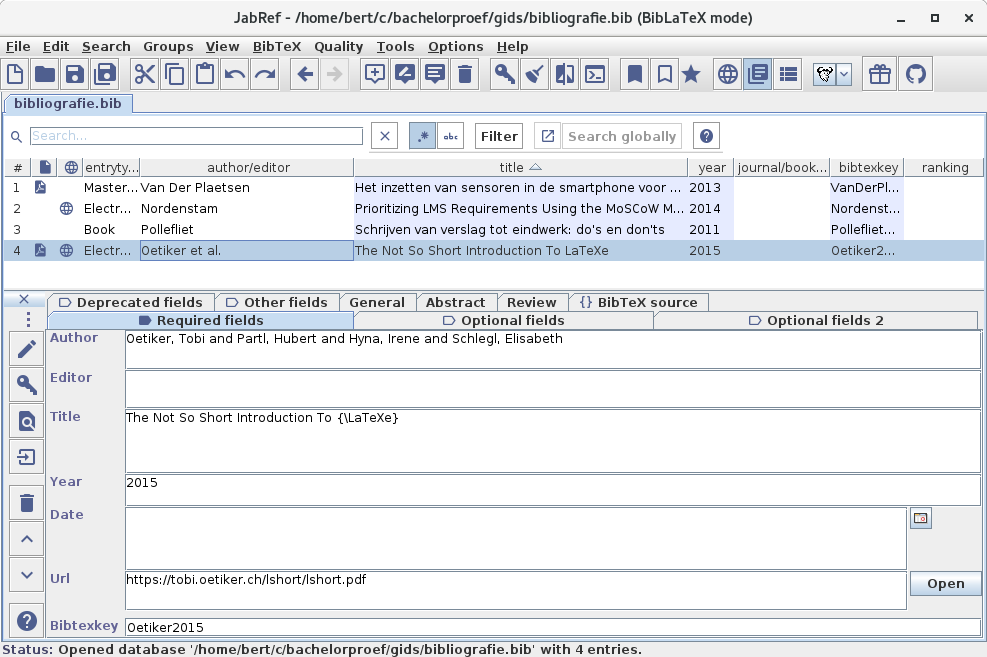
\includegraphics[width=\linewidth]{jabref-screenshot}
  \caption[Jabref]{\textbf{Jabref.} Centraal in de gebruikersinterface vind je een \emph{overzicht} van de verschillende bronnen in deze bibliografische databank, in dit geval vier. De \emph{pdf-icoontjes} links bij de eerste en vierde bron geven aan dat de bron lokaal opgeslagen is als pdf. Als je er op klikt, wordt de pdf geopend. De \emph{wereldbol-icoontjes} bij de tweede en vierde bron duiden op een url die je in de webbrowser kan openen als je er op klikt. Onderaan bevindt zich een \emph{detailvenster} met de bijgehouden gegevens voor de vierde bron. Deze worden opgedeeld in verschillende tabbladen, o.a.~verplichte gegevens (``Required fields'', optionele (``Optional'' en ``Other fields''), enz. In dit geval zijn de namen van de auteurs ingevuld (zie Sectie~\ref{sub:algemene_bibliografische_gegevens}). Er zijn in dit geval geen redacteurs (``Editors''), en dat veld is dan ook leeg gebleven. Het veld ``Bibtexkey'' onderaan is automatisch gegenereerd (zie Sectie~\ref{sub:jabref_instellingen}) door te klikken op het \emph{sleutelsymbool} in de knoppenbalk links.}
  \label{fig:jabref}
\end{figure}

\subsection{JabRef instellingen}
\label{sub:jabref_instellingen}

Je kan Jabref downloaden van \url{http://www.jabref.org/} en installeren op zowel Windows, MacOS als Linux. Bij het voor de eerste keer opstarten is het nuttig om volgende instellingen aan te passen:

\begin{itemize}
  \item Kies in het menu voor File > Switch to BibLaTeX mode. Dit maakt de bestandsindeling van de bibliografische databank compatibel met het aangeboden {\LaTeX}-sjabloon voor de bachelorproef.
  \item Kies in het menu voor Options > Preferences en dan voor de categorie ``BibTeX key generator''. Elke bron in de databank wordt geïdentificeerd door een unieke sleutel die je kan automatisch laten genereren. Je kan de vorm ervan zelf instellen. Het standaardformaat is de familienaam van de eerste auteur gevolgd door het publicatiejaar, bv. ``Knuth1998''. Je kan dit naar eigen smaak aanpassen, maar kies dit vooraf en hou je er aan. Je zal deze sleutel gebruiken om vanuit de tekst te verwijzen naar je bronnen, bv. met het commando \verb|\parencite{Knuth1998}|.
  \item Kies in het Preferences-venster voor de categorie File en geef een directory op voor het bijhouden van PDFs van de gevonden bronnen onder ``Main file directory''. Het is heel interessant om de gevonden artikels te downloaden en onder die directory bij te houden. Nog beter is om als naam van het bestand de BibTeX key te nemen (bv. Knuth1998.pdf). Je kan het bestand dan makkelijk openen vanuit Jabref.
\end{itemize}

Je kan de andere instellingen nakijken en eventueel naar wens aanpassen, maar de hierboven opgesomde zijn de belangrijkste.

\subsection{Algemene bibliografische gegevens}
\label{sub:algemene_bibliografische_gegevens}

De bedoeling van een bibliografie is de lezer toelaten je bronnen zelf op te zoeken en te beoordelen op betrouwbaarheid. Dat betekent dat je voldoende informatie moet opgeven zodat de bron terug te vinden is. Afhankelijk van het soort bron (artikel in een journal, boek, website, enz.) moet je andere informatie opgeven. Dit wordt verderop uitgediept. Drie elementen zijn sowieso \emph{altijd} essentieel: de auteur, de titel van de bron en het jaar (of datum) van publicatie. Als één van deze drie ontbreekt, wordt het bijzonder moeilijk om de oorsprong en de kwaliteit van de bron te evalueren. Dit soort bronnen kan je bijhouden ter info, maar zijn niet geschikt om op te nemen in een bibliografie. Als de auteur onbekend is, is het niet immers mogelijk om te beoordelen of die wel de autoriteit heeft om op een objectieve en diepgaande manier over het onderwerp te schrijven. Als het jaartal niet opgegeven is, is het erg moeilijk om na te gaan in hoeverre deze bron nog niet achterhaald is door recentere ontwikkelingen in het vakgebied.

Enkele tips bij het invullen van auteursnamen:

\begin{itemize}
  \item Noteer de naam van auteurs in de vorm ``Familienaam, Voorna(a)m(en)''. Dus ``Van Vreckem, Bert'' en niet ``Bert Van Vreckem.'' In principe wordt de tweede notatie ook aanvaard, maar dit werkt enkel voor typische angelsaksische namen met een tweede voornaam (bv. ``Donald Ervin Knuth''). De eerste twee woorden worden beschouwd als voornamen, het laatste woord als de familienaam. ``Van'' wordt in dat geval dus verkeerdelijk beschouwd als tweede voornaam.
  \item Als de auteur een bedrijf of organisatie is, met een naam bestaande uit verschillende woorden, zet die dan tussen accolades: bv. ``\{The Linux Foundation\}''. Zoniet probeert {\LaTeX} dit als een persoonsnaam te interpreteren. ``Foundation'' wordt dan de familienaam, ``The'' en ``Linux'' de twee voornamen.
  \item Als je meerdere auteurs hebt, scheid elke naam dan met \texttt{and}, bv. ``Bernard, Anita and Buysse, Jens and Van Vreckem, Bert''.
  \item Na invullen van de auteursna(a)m(en) klik je op de knop met het sleutel-icoon (zie Figuur~\ref{fig:jabref}) om een unieke sleutel te genereren voor deze bron.
  \item Naast een auteurveld is er ook een veld voor eventuele redacteur(en) (\emph{editor}) voorzien. Minstens één van de twee moet ingevuld zijn, soms allebei. Dit gebeurt bijvoorbeeld in een boek dat samengesteld is uit hoofdstukken die telkens door andere auteurs geschreven zijn en waar je naar één bepaald hoofdstuk wil verwijzen. Verderop vind je daar een voorbeeld van.
\end{itemize}

Merk trouwens op dat in een bibliografie \textbf{enkel werken mogen opgenomen zijn waarnaar verwezen wordt vanuit de tekst}. {\LaTeX} doet dit standaard automatisch, dus als je bronnen in de lijst mist, dan betekent dit dat je die niet in de tekst gebruikt hebt.

Probeer telkens zoveel mogelijk informatie bij te houden over je bronnen, zodat het later makkelijker wordt die terug te vinden. Dit is een tijdrovend proces, en niet al deze informatie wordt ook in de bibliografie opgenomen. Het raadplegen van de databank wordt wel een stuk makkelijker. Heb hier voldoende aandacht voor en controleer ook goed het resultaat in de bibliografie zelf. Zijn de auteurs correct weergegeven? Heb je een jaartal? Is er voor een online bron (zie verder) een URL en datum van raadplegen opgegeven? Enz.

Enkele velden die zinvol zijn om altijd trachten in te vullen:

\begin{description}
  \item[Abstract] Samenvatting van het artikel. Dit is meestal de eerste paragraaf van een artikel en wordt altijd duidelijk aangegeven.
  \item[DOI] of ``Digital Object Identifier''. Dit is een unieke code voor artikels in wetenschappelijke publicaties die het opzoeken makkelijker maakt (op voorwaarde dat de DOI gegeven is).
  \item[File] Naam van het bestand met het gedownloade artikel. Je kan vanuit JabRef het artikel openen in een PDF-viewer of desgevallend tekstverwerker.
  \item[Keywords] Kernwoorden die het onderwerp weergeven, gescheiden door komma's.
  \item[Review] Je eigen opmerkingen over deze bron. Waarom heb je deze bijgehouden? Wat is het interessantste dat je er uit geleerd hebt?
  \item[URL] De URL waar je het artikel gevonden hebt. Deze URL wordt niet altijd in de bibliografie opgenomen, maar is altijd nuttig om bij te houden. Je kan vanuit JabRef de website openen in een webbrowser.
  \item[Urldate] de datum waarop je deze bron het laatst hebt geraadpleegd.
\end{description}

\subsection{Specifieke bibliografische gegevens}
\label{sub:specifieke_bibliografische_gegevens}

In deze sectie wordt voor de meest relevante soorten bronnen uitgelegd hoe deze correct bij te houden en in de bibliografie op te nemen. JabRef geeft zelf al enige aanwijzingen over welke informatie minstens nodig is: in het detailvenster (zie Afbeelding~\ref{fig:jabref}) moet je minstens het tabblad ``Required fields'' invullen. Voor elke soort publicatie (zie Sectie~\ref{sub:publicatievormen}) vind je verderop een overzicht van de in te vullen velden en wat die precies betekenen, en hoe de referentie in de literatuurlijst er uit zal zien.

Bij het toevoegen van een nieuwe bron aan een bibliografische databank moet je eerst het type selecteren (zie Afbeelding~\ref{fig:jabref-entrytypes}). Hieronder bespreken we enkel de belangrijkste die relevant zijn voor een bachelorproef.

\begin{figure}
  \centering
  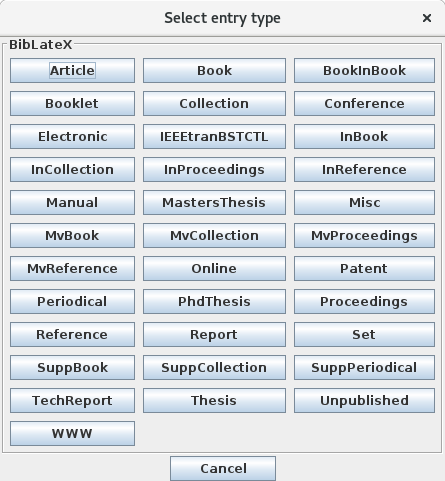
\includegraphics[width=0.6\linewidth]{img/jabref-entrytypes}
  \caption[Soorten bronnen in JabRef]{\textbf{Soorten bronnen in Jabref.} Bij het toevoegen van een nieuwe bron in JabRef (Ctrl+N) moet je eerst het soort publicatie kiezen. Afhankelijk van het soort moet in de literatuurlijst immers andere informatie gegeven worden.}
  \label{fig:jabref-entrytypes}
\end{figure}

\paragraph{Article}

Dit soort bron wordt enkel gebruikt voor artikels die verschenen zijn in een wetenschappelijke journal. Artikels in (vak)tijdschriften of kranten vallen hier \emph{niet} onder. Verplichte velden:

\begin{description}
\item[Author] De naam van de auteur;
\item[Title] De titel van het artikel;
\item[Year] Jaar waarin het artikel verschenen is;
\item[Volume] De jaargang van het tijdschrift waarin het artikel verschenen is;
\item[Number] Het nummer (binnen de jaargang) waarin het artikel verschenen is (soms niet gegeven);
\item[Pages] Paginanummers
\end{description}

Voorbeeld:
\begin{verbatim}
@Article{SabiEtAl2016,
  author       = {Sabi, Humphrey M. and Uzoka, Faith-Michael E. and Langmia,
                  Kehbuma and Njeh, Felix M.},
  title        = {Conceptualizing a model for adoption of cloud computing in
                  education},
  journaltitle = {International Journal of Information Management},
  year         = {2016},
  volume       = {36},
  number       = {2},
  pages        = {183--191},
  doi          = {10.1016/j.ijinfomgt.2015.11.010},
  url          = {http://www.sciencedirect.com/science/article/pii/S0268401215001115},
  abstract     = {Cloud computing is a pervasive computing paradigm that [...]},
  keywords     = {Cloud computing, Educational technologies, [...]},
  owner        = {bert},
  timestamp    = {2016-09-01},
}
\end{verbatim}

In de bibliografie ziet dit er zo uit: \fullcitebib{SabiEtAl2016}

\paragraph{InProceedings}

Dit soort bron wordt gebruikt voor artikels die gepubliceerd zijn in het verslag (proceedings) van een \emph{wetenschappelijke} conferentie. Verplichte velden:

\begin{description}
  \item[Author] Naam van de auteur(s),
  \item[Title] Titel van het artikel,
  \item[Booktitle] De naam van de conferentie,
  \item[Year] Het jaar waarin de conferentie doorging.
\end{description}

Daarnaast kan je optioneel ook volgende velden invullen:

\begin{description}
  \item[URL] naar de website van de conferentie waar het artikel kan gevonden (eventueel rechtstreeks naar de pdf);
  \item[Urldate] datum waarop je deze bron het laatst geraadpleegd hebt.
  \item[DOI] op voorwaarde dat er één toegewezen is aan dit artikel.
\end{description}

Voorbeeld:
\begin{verbatim}
@InProceedings{VanVreckemEtAl2013,
  author    = {Van Vreckem, Bert and Borodin, Dmitriy and De Bruyn, Wim and
               Now\'{e}, Ann},
  title     = {A Reinforcement Learning Approach to Solving Hybrid Flexible
               Flowline Scheduling Problems},
  booktitle = {Multidisciplinary International Scheduling Conference (MISTA)
               2013},
  year      = {2013},
  url       = {https://expertise.hogent.be/files/10711623/hffsp_la.pdf},
  urldate   = {2016-09-01},
  abstract  = {In this paper, we present a method based on Learning Automata to
               solve Hybrid Flexible Flowline Scheduling Problems [...].},
  owner     = {bert},
  timestamp = {2016-09-01},
}
\end{verbatim}

In de bibliografie: \fullcitebib{VanVreckemEtAl2013}

\paragraph{InBook}

Dit type gebruik je als je wil verwijzen naar een specifiek hoofdstuk in een boek. Minstens volgende velden moeten dan ingevuld zijn:

\begin{description}
  \item[Author] De auteur(s) van het hoofdstuk,
  \item[Editor] De redacteur(en) van het boek (indien van toepassing),
  \item[Year] Jaartal waarin het boek werd uitgegeven,
  \item[Title] Titel van het \emph{hoofdstuk},
  \item[Pages] Begin- en eindpagina van het hoofdstuk,
  \item[Booktitle] Titel van het \emph{boek},
  \item[Publisher] Naam van de uitgeverij.
\end{description}

Optioneel kan je ook volgende informatie aanvullen:

\begin{description}
  \item[Subtitle of Booksubtitle] ondertitel van het hoofdstuk of boek, resp.,
  \item[Edition] Nummer van de uitgave,
  \item[Location] Stad waar de uitgeverij gevestigd is,
  \item[ISBN] Het ISBN-nummer van het boek (ter info, wordt nooit getoond in de bibliografie).
\end{description}

Bij een boek is het ongebruikelijk om een URL op te geven. Als je bijvoorbeeld ter info voor jezelf de URL van het boek op de website van de uitgever wil bijhouden, doe je dit best in een ander veld, bv. Comment of Review.

Voorbeeld
\begin{verbatim}
@InBook{Meyr2008,
  author       = {Meyr, Herbert},
  title        = {Forecast Methods},
  booktitle    = {Supply Chain Management and Advanced Planning},
  year         = {2008},
  editor       = {Stadtler, Hartmut and Kilger, Christoph},
  booksubtitle = {Concepts, Models, Software, and Case Studies},
  edition      = {4e editie},
  publisher    = {Springer},
  location     = {Heidelberg},
  isbn         = {978-3-540-24814-9},
  pages        = {461--472},
  comment      = {https://www.springer.com/us/book/9783540248149},
  owner        = {bert},
  timestamp    = {2016-09-02},
}
\end{verbatim}


In de bibliografie: \fullcitebib{Meyr2008}

%% TODO: boek, thesis, manual, \ldots

\paragraph{Electronic of Online}

Onder dit type publicatie vallen vrijwel alle online bronnen die niet onder een andere categorie te plaatsen zijn: blogartikels, artikels in online vaktijdschriften of portaalsites, Youtube-video's van presentaties op vakconferenties, online documentatie, enz.

Merk op dat je de algemene website van organisaties, softwarepakketten, enz. \emph{niet} in je literatuurlijst mag opnemen. Deze kan je wel in een voetnoot zetten.

Deze velden moet je verplicht invullen:

\begin{description}
  \item[Author] Auteur(s) van de bron, spreker (in het geval van een video van een lezing op een conferentie), \ldots
  \item[Title] Titel van de bron, lezing, \ldots
  \item[Year] Jaartal van publicatie (of eventueel \textbf{Date}, de dag van publicatie, als die bekend is),
  \item[URL] naar de website waar de bron kan teruggevonden worden,
  \item[Urldate] Datum van laatste raadplegen,
\end{description}

Bij dit soort bronnen worden veel fouten gemaakt bij het refereren. Het is essentieel dat de URL wordt meegegeven en ook de datum van raadplegen. Het web is voortdurend in beweging, en het is mogelijk dat de inhoud van een webpagina in de loop van de tijd verandert (bv. fouten die verbeterd worden) of zelfs dat een website herstructureert en de URL dus op een gegeven manier niet meer geldig is. Door de datum van raadplegen op te geven, bied je de lezer nog de kans om terug te vinden hoe die website er op dat moment in de tijd uitzag, via bijvoorbeeld de Wayback Machine van het Internet Archive\footnote{\url{https://archive.org/web/}}.

Voorbeeld van een blogartikel:

\begin{verbatim}
@Electronic{LewisFowler2014,
  author    = {Lewis, James and Fowler, Martin},
  title     = {Microservices: a definition of this new architectural term},
  date      = {2014-03-25},
  url       = {http://martinfowler.com/articles/microservices.html},
  urldate   = {2016-09-01},
  abstract  = {The term "Microservice Architecture" has sprung up over [...]},
  keywords  = {application architecture, web services, microservices},
  owner     = {bert},
  timestamp = {2016-09-01},
}
\end{verbatim}

In de bibliografie wordt dit: \fullcitebib{LewisFowler2014}

Een ander voorbeeld, deze keer van een presentatie op een vakconferentie die op Youtube is gepubliceerd. Omdat er niet meteen een apart veld voorzien is voor het vermelden van de naam van de conferentie, is die hier in het titelveld verwerkt.

\begin{verbatim}
@Online{Hykes2013,
  author       = {Solomon Hykes},
  title        = {The future of Linux Containers (PyCon 2013)},
  date         = {2013-03-21},
  url          = {https://www.youtube.com/watch?v=wW9CAH9nSLs},
  urldate      = {2016-09-01},
  abstract     = {At PyCon Solomon Hykes shows docker to the public for the
                  first time.},
  owner        = {bert},
  timestamp    = {2016-09-01},
}
\end{verbatim}

In de bibliografie: \fullcitebib{Hykes2013}

\section{Op zoek naar relevante informatie}
\label{sec:op_zoek_naar_relevante_informatie}

Via de HoGent bib krijg je toegang tot een grote hoeveelheid wetenschappelijke en vakliteratuur die niet publiek beschikbaar zijn.
% Zoek naar scripties, thesissen, bachelorproeven van vorige jaren over je onderwerp. http://bib.hogent.be/zoeken/scripties-hogent/
% Log in op Apollo (https://apollo.hogent.be/, via VPN) voor toegang tot databanken die niet publiek beschikbaar zijn. In het bijzonder Elsevier ScienceDirect, Springer Online Journals, en Web of Science zijn voor ons vakgebied het interessantst.
% Vanuit Apollo kan je ook Google Scholar lanceren. Dat kan ook via het publieke internet, maar dan heb je geen toegang tot bepaalde bronnen. Scholar kent de abonnementen waar de bib op is ingeschreven en kan op die manier toegang geven tot artikels die niet publiek toegankelijk zijn.
% Springer eBooks http://bib.hogent.be/zoeken/ebooks/ is een verzameling van boeken uitgegeven door Springer, met o.a. een uitgebreid aanbod binnen computerwetenschappen.
% Via het publieke internet vind je uiteraard ook veel informatie.
% Wikipedia is een goed startpunt, maar vergeet niet dat Wikipedia-artikels op zich niet kunnen als referenties. Bekijk de oorspronkelijke bronnen van het artikel.
% Arxiv.org is een database van Open Acces artikels in een hele reeks onderzoeksdomeinen, o.a. de Computing Research Repository http://arxiv.org/corr/home
% Ga op zoek naar presentaties op vakconferenties rond je onderwerp (vb. Google IO, WWDC, http://lanyrd.com/topics/android/, \ldots). Tegenwoordig worden vele conferenties gefilmd en achteraf gepubliceerd op Youtube of Vimeo
% Er bestaan verschillende portaalsites voor actuele ict-gerelateerde onderwerpen waar technische artikels, presentaties, interviews, enz. op verschijnen, bv. dzone.com, infoq.com, enz.
% Wie zijn de belangrijkste namen in de ``community''? Keynote-speakers op conferenties, auteurs van de belangrijkste boeken over het onderwerp, enz. Volg deze personen op Twitter, zoek uit of ze een blog hebben, actief zijn op LinkedIn, enz. Lees al wat je kan vinden dat ze geschreven hebben de laatste jaren.
%
% XXX: SECTIE: de literatuurstudie schrijven
% Hoort misschien thuis in ``schrijven''???
%
% De literatuurstudie/state-of-the-art is een doorlopende tekst waarin je in je eigen woorden de situatie in het onderzoeksdomein schetst, met op gepaste plaatsen verwijzingen naar de literatuur. Expliciet schrijven ``in het artikel X van Y heb ik Z gelezen'' wordt niet gedaan. Lees een aantal wetenschappelijke publicaties over je onderwerp en probeer die stijl na te volgen.
%
% Wanneer verwijzen naar de literatuur:
% - Elke introductie van domeinspecifieke vaktermen
% - Elke bewering over het vakdomein (die je quantificeert!)
% - Elke verwijzing naar resultaten vorig onderzoek
%
% Twee commando's: (Auteur, jaar) of Auteur (jaar)

% TODO: samenvatting
%
% - Doelstelling literatuurstudie
% - enkel secundaire bronnen/publicaties
% - Gebruik JabRef en vul de juiste info in
% - Ga op de juiste plaatsen op zoek naar informatie en doe de CRAP test bij elke bron
% - Schrijf de literatuurstudie (typisch het inleidende hoofdstuk) als een doorlopende en samenhangende tekst waarin je in je eigen woorde de state-of-the-art in je onderzoeksdomein schetst. Verwijs op gepaste plaatsen naar de literatuur.

\section{Samenvatting}
\label{sec:literatuuronderzoek_samenvatting}

\begin{itemize}
  \item Er zijn drie soorten bronnen: primaire (resultaten van eigen onderzoek), secundaire (publicaties in wetenschappelijke of vakliteratuur) en tertiaire (encyclopedieën en zoekindexen).
  \item In een bibliografie horen enkel \emph{secundaire} bronnen thuis.
  \item Zet je bibliografische databank op (bv. met Jabref) voordat je op zoek gaat naar informatie over je onderwerp en hou van wat je vindt nauwgezet zoveel mogelijk informatie bij.
  \item Zorg dat je altijd minstens de auteur, titel en jaartal hebt en daarnaast minstens alle andere verplichte informatie correct noteert.
\end{itemize}

\chapter{Onderzoeksmethoden}
\label{ch:onderzoeksmethoden}

In dit onderwerp vind je aanbevelingen in verband met een aantal vaak gebruikte onderzoeksmethoden. Meer bepaald bespreken we de aanpak van een vergelijkende studie, hoe je correct experimenten opzet en hoe je op een correcte manier rapporteert over bekomen resultaten (in het bijzonder cijfermateriaal).

\section{De vergelijkende studie}
\label{sec:vergelijkende-studie}

Een type onderwerp dat vaak gekozen wordt voor een bachelorproef is een vergelijkende studie. Je bent op zoek naar een oplossing voor een probleem in de vorm van een software- of hardware-product, platform, dienst, enz. De bedoeling van de studie is om alle mogelijke alternatieven naast elkaar te zetten en een keuze te maken over de meest geschikte.

De ervaring leert dat een vergelijkende studie pas echt goed is als er een concreet doel is, een reële situatie waar de geselecteerde oplossing ook werkelijk zal toegepast worden. Het gevaar bestaat dat de studie zich beperkt tot het achter elkaar opsommen van enkele arbitrair gekozen mogelijkheden. Er volgt een paragraafje uitleg, soms gewoon van Wikipedia gehaald, met een opsomming van wat voor- en nadelen, maar niet gestructureerd en zonder rode draad. Een bepaald aspect als ``gebruiksvriendelijkheid'' wordt dan bijvoorbeeld in één product besproken, maar niet voor de andere, enz. De eigen inbreng is dan miniem: een dagje zoeken op Wikipedia, samenvatten of verder uitschrijven, klaar. Dit is op zich dus onvoldoende.

Maar hoe pak je het dan \emph{wel} aan?

Laat ons veronderstellen dat je na je afstuderen aan de slag wil als webontwikkelaar, en je bent op zoek naar een geschikt PHP-framework om je websites mee te bouwen.

\subsection{Requirements-analyse}
\label{ssec:requirements-analyse}

Om een goede keuze te maken begin je met het verzamelen van \emph{requirements}, zowel \textit{functionele} als \emph{niet-functionele}, bijvoorbeeld:

\begin{itemize}
\item Functionele requirements
  \begin{itemize}
  \item Ondersteuning voor HTML5/CSS3
  \item Responsive design
  \item Er moet een authenticatiemodule in zitten dat OpenID, Facebook- en Google-authenticatie ondersteunt
  \item \ldots
  \end{itemize}
\item Niet-functionele requirements
  \begin{itemize}
  \item Moet bestand zijn tegen de top-10 beveiligingsproblemen van OWASP\footnote{\url{https://www.owasp.org/index.php/Category:OWASP_Top_Ten_Project}}
  \item Wachtwoorden worden opgeslagen volgens de state-of-the art (\emph{salted} en \emph{hashed})
  \item Moet open source zijn
  \item Moet gratis zijn
  \item \ldots
  \end{itemize}
\end{itemize}

Als je het onderzoek doet voor een ``klant'' (= je co-promotor), dan betrek je uiteraard alle belanghebbenden bij dit proces! Je lijst de requirements op en verdeelt ze onder naar belangrijkheid, bijvoorbeeld via de MoSCoW-techniek~\parencite{Nordenstam2014}. Je verdeelt de requirements dan in categorieën zoals ``must-have'', ``should-have'' en ``nice-to-have''.

\subsection{Long list}
\label{ssec:long-list}

Dan zoek je \emph{zoveel mogelijk} alternatieven die in aanmerking komen om gebruikt te worden, m.a.w.~al diegenen die je kan vinden. Je noemt ze in deze \emph{long list} (die soms kan bestaan uit tientallen alternatieven) bij naam, met eventueel vermelding van een website en een beschrijving in één zin. Elk alternatief toets je af aan de requirements, voor zover dit al mogelijk is aan de hand van informatie die je op de website vindt of via andere bronnen. Zaken die je niet kan verifiëren laat je gewoon open om later na te kijken of misschien zelfs te negeren (als het bv.~gaat om een onbelangrijke feature, of als verschillende andere must-haves niet voldaan zijn). Je sorteert de long list dan volgens het aantal voldane requirements, en maakt hier een overzichtelijke tabel van. Hopelijk heb je een aantal alternatieven overgehouden die voldoen aan alle must-haves en zoveel mogelijk should-haves en nice-to-haves.

\subsection{Short list en proof-of-concept}
\label{ssec:short-list-poc}

 De meest veelbelovende alternatieven weerhoud je voor de volgende fase. De alternatieven in deze \emph{short list} ga je in meer detail bespreken en verder tegenover elkaar afwegen. Zet eventueel een \emph{proof-of-concept} op, waarin je één of enkele van de meest veelbelovende alternatieven uitprobeert aan de hand van eenzelfde vastgelegd \emph{scenario} waarin je de requirements die je nog niet hebt kunnen verifiëren aan bod laat komen.

\subsection{Conclusie}
\label{ssec:vgl-studie-conclusie}

Tenslotte geef je je \emph{aanbeveling}, het alternatief dat het beste aansluit bij de requirements, en wat eventueel nog moet gedaan worden om het nog beter geschikt te maken.

\section{Experimenten opzetten}
\label{sec:experimenten-opzetten}

% TODO
% Belangrijk: reproduceerbaar aan de hand van de beschrijving
% => voldoende detail om te kunnen nabootsen
% Gebruikte hardware, software
% Procedure opzetten testomgeving (afbeelding!)

\section{Cijfermateriaal rapporteren}
\label{sec:cijfermateriaal}

% TODO
% vb. performantievergelijking
% - vergelijk je de juiste dingen? Zijn neveneffecten uitgeschakeld?
% - Experimenten vele keren herhalen
% - Enkel gemiddeldes vermelden is onvoldoende! Minstens ook standaardafwijkingen geven en statistische toetsen uitvoeren om te verifiëren of resultaten significant verschillen.



\chapter{De bachelorproef schrijven}
\label{ch:schrijven}

Op een bepaald moment heb je een heleboel informatie verzameld en geanalyseerd, en wordt het tijd om het finale document op te maken. In dit hoofdstuk vind je enkele tips en richtlijnen om tot een goed resultaat te komen.

In deze gids beperken we ons tot enkele belangrijke punten en specifieke aanbevelingen voor de opmaak van de tekst in {\LaTeX}. Een meer omvattend overzicht kan je o.a.~vinden in het boek van~\textcite{Pollefliet2011}.

\section{Algemene richtlijnen}
\label{ch:algemene-richtlijnen}

Wanneer je een tekst schrijft wil je uiteraard je best doen om deze zo aangenaam mogelijk te maken om te lezen. Er zijn echter een aantal dingen waar je moet op letten. In je bachelorproef toon je aan dat je een professionele instelling hebt en een gezonde dosis maturiteit op zak hebt. Dat moet ook tot uiting komen in je schrijfstijl. De tekst moet professioneel en objectief overkomen. Vermijd in het bijzonder volgende zaken:

\begin{itemize}
  \item Schrijven vanuit je eigen standpunt is uit den boze. Gebruik dus nooit de \textbf{ik-vorm}. Die geeft immers de indruk dat je je \emph{eigen mening} geeft, en als junior in je vakgebied heb je daarvoor onvoldoende autoriteit. De beweringen die je in je bachelorproef doet moeten objectieve aantoonbare feiten zijn.
  \item Gebruik geen \textbf{spreektaal}. Blijf formeel en zakelijk.
  \item Gebruik geen \textbf{vage termen} om een hoeveelheid aan te duiden, bv. lang, groot, snel, populair, \ldots Quantificeer al deze uitspraken met cijfers en meeteenheiden (uiteraard ondersteund door literatuurverwijzingen of resultaten van eigen onderzoek).
  \item Gebruik geen \textbf{toekomstige tijd.} Op het moment dat je afgewerkte bachelorproef gelezen wordt, is het een verslag van in het verleden uitgevoerd onderzoek. Dus niet ``Eerst zal worden gekeken naar\ldots'' maar ``Eerst werd onderzocht\ldots''
\end{itemize}

% http://www.taalwinkel.nl/schrijfproces/een-wetenschappelijke-schrijfstijl/
% familiair (je), ``populariserend''
% Vermijd passieve zinnen, die maken de tekst vager en dubbelzinniger

% Voorbeeld vage termen:
% ``Doorheen de laatste jaren zijn mobiele applicaties enorm ge-
% groeid''
% Bron -> http://blog.appfigures.com/app-stores-growth-accelerates-in-2014/
% Gebruik waar mogelijk Nederlandse termen en vermijd Anglicanismen. Als er een Nederlands woord voor bestaat gebruik je dat, en niet de Engelse term. Bv. tree -> boom, deployen -> uitrollen, enz.

% Een zin = een gedachte
% Een paragraaf = bij elkaar horende gedachten die één onderwerp, redenering vormen
% Tip: De eerste zin van een paragraaf bevat de hoofdgedachte van de paragraaf, de andere zinnen leggen die verder uit, of gaan er dieper op in.
%
% Samengestelde woorden hangen aan elkaar: informatiebeveiliging ipv informatie beveiliging

Hou rekening met je \emph{doelpubliek}. In principe kan je er van uitgaan dat de lezer een ict-achtergrond heeft (tenzij je je onderwerp uitwerkt in samenwerking met of in opdracht van iemand uit een andere discipline). Je kan dus meestal een zekere basiskennis veronderstellen, maar termen en afkortingen die specifiek zijn voor je eigen onderzoeksdomein moet je zeker uitleggen.

Doe een \emph{grondige controle} op spellings- en grammaticale fouten. Deze \emph{moeten} er uit zijn bij indienen. Voor een informaticus telt elke punt en komma. Een tekst vol fouten een heel slechte indruk over je capaciteiten.

Begin elk hoofstuk (en sectie) met een inleidende paragraaf die aangeeft wat de inhoud ervan is wat de link is met het vorige hoofdstuk. Iemand die meteen dat hoofdstuk begint te lezen krijgt op die manier wat context.


% Volgorde van schrijven (samenvatting laatste)

%- Conclusie, samenvatting, voorwoord schrijf je het laatste maar het is vaak het eerste dat gelezen wordt. Bijzonder veel aandacht aan schenken
    %- Conclusie moet terug grijpen op de onderzoeksvraag
    %- Bedenkingen, future work
    %- Samenvatting is geen voorwoord. Moet maw. ook belangrijkste conclusies bevatten

\section{Structuur}
\label{sec:structuur}

% Titel:
% - concreet, niet enkel het onderzoeksdomein benoemen
% - Geef het onderwerp, niet een onderzoeksvraag
% - Gebruik geen afkortingen en vermijd jargon
% - Vermijd algemene, nietszeggende woorden. vb. ``Studie,''  ``Onderzoek naar'' -> een bachelorproef is altijd een onderzoek


\section{Afbeeldingen}
\label{sec:afbeeldingen}

Het invoegen van afbeeldingen in een {\LaTeX}-document is \'e\'en van de struikelblokken voor beginnende gebruikers van het tekstzetsysteem. In een klassieke WYSIWYG tekstverwerker ben je gewend om zelf te bepalen waar een afbeelding op het papier terecht zal komen. Meestal doe je dat dan meteen onder het deel van de tekst waar naar de afbeelding verwezen wordt. In een groter document wordt dit problematisch. Het is immers mogelijk dat door toevoegingen van tekst vóór de afbeelding, die de ondermarge gaat overschrijden. De tekstverwerker zal dan wellicht de afbeelding naar de volgende bladzijde verplaatsen en je krijgt onderaan extra witruimte. Dit ziet er niet goed uit, en je verliest dan kostbare tijd met het goed positioneren van de afbeeldingen ten opzichte van de tekst.

{\LaTeX} kan zelf bepalen waar een afbeelding het best gepositioneerd wordt. Het is in eerste instantie vervelend om deze controle te moeten afstaan, maar het document zal er wel een stuk beter door uitzien. Soms kiest {\LaTeX} er voor om de afbeelding een bladzijde verder of eerder te plaatsen dan de tekst die er op betrekking heeft. Dat betekent dus dat de context voor de afbeelding niet meer bij de afbeelding staat. Dit kan je echter oplossen door bij elke afbeelding een bijschrift (\emph{caption}) te plaatsen dat volledig beschrijft wat er op de afbeelding te zien is. Beperk je niet tot enkele woorden. Gebruik volledige zinnen zodat de lezer de afbeelding kan begrijpen zonder naar de bijhorende tekst te moeten gaan zoeken. In de tekst zelf verwijs je dan uiteraard naar de afbeelding (met \verb|\ref{fig:label}|).

% TODO: template voor invoegen van afbeelding

Onder de auteurswetgeving is het toegelaten om binnen de context van onderwijs afbeeldingen uit andere publicaties over te nemen zonder voorafgaande toestemming van de auteur.Het is dan uiteraard essentieel dat je in het bijschrift een literatuurverwijzing toevoegt. Zoniet wordt dit beschouwd als plagiaat.

Logo's van producten of bedrijven toevoegen is \emph{geen} goed idee. Dit valt immers niet enkel onder de auteurswetgeving, maar onder de merkenwet. Een logo weerspiegelt de identiteit van een bedrijf en het gebruik van het logo wordt dan ook sterk gecontroleerd (grootte, correct kleurgebruik, enz.). Derden mogen enkel na expliciete toestemming en onder specifieke voorwaarden het logo gebruiken. In een thesis voegt een logo trouwens geen enkele inhoudelijke meerwaarde toe, wat op zich al een reden is om er geen in te voegen.

Wanneer je een afbeelding overneemt van een website, zorg er dan zeker voor dat de resolutie voldoende hoog is. Afbeeldingen die er op een beeldscherm goed uitzien, kunnen op papier duidelijk de individuele pixels zichtbaar worden, wat niet goed overkomt. Een beeldscherm heeft typisch een veel lagere resolutie (96 DPI of \emph{dots per inch}, beeldpunten per duim) dan een printer (300 of 600 DPI). Voor een goed resultaat moet een afbeelding minstens evenveel pixels bevatten als de gewenste hoogte of breedte van de afbeelding op papier, vermenigvuldigd met de resolutie. Als je dus bijvoorbeeld een afbeelding op $5 \times 5$ cm (of ongeveer 2 inch) wil afdrukken op een 300 DPI printer, moet je afbeelding minstens $600 \times 600$ pixels groot zijn.

Een alternatief is werken met \emph{vector graphics}, m.a.w.~figuren die in het document getekend worden aan de hand van wiskundig gedefinieerde vormen. Er bestaat een zeer uitgebreide package voor {\LaTeX} hiervoor: Ti$k$Z. Dit heeft wel een steile leercurve, maar het resultaat is wel van hoge kwaliteit. Een inleiding op Ti$k$Z valt buiten de scope van deze gids, maar er zijn veel tutorials en voorbeelden te vinden op het Internet\footnote{Bijvoorbeeld \url{http://www.texample.net/tikz/}}.


% Voldoende hoge resolutie voor screenshots (gekopieerd van webpagina): http://brandonmathis.com/blog/2010/10/08/how-to-get-high-resolution-screenshots-of-a-website
% Kleurenpallet (contrast, toeg
% tikz (maar dat is een specialiteit op zich\ldots)
%
% Index? Woordenlijst?


\appendix

\bibliographystyle{apacite}
\bibliography{bachproef-gids}

\end{document}

